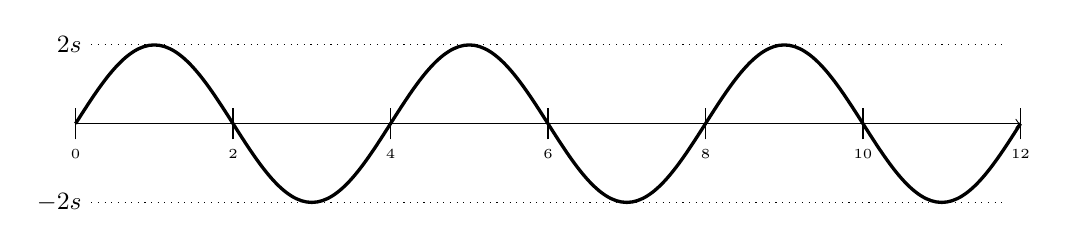
\begin{tikzpicture}[domain=0:4]
%    \begin{axis}[
%		xlabel=$x$,
%		ylabel={$f(x) = x^2 - x +4$}
%	]
%	% use TeX as calculator:
%	\addplot {sin(x)};
%	\end{axis}
    \draw[->] (0,0) -- (12,0);
    \draw[dotted] (0.2,1)node[left,font=\small] {$2s$} -- (11.8,1);
    \draw[dotted] (0.2,-1)node[left,font=\small] {$-2s$} -- (11.8,-1); 
    \foreach \x in {0,2,...,12}{
    \draw (\x,-0.2)node [below,font=\tiny,] {\x} -- (\x,0.2) ;
    }
    \draw[very thick] (0,0) sin ++(1,1) cos ++(1,-1) sin ++(1,-1) cos ++(1,1) sin ++(1,1) cos ++(1,-1) sin ++(1,-1) cos ++(1,1) sin ++(1,1) cos ++(1,-1) sin ++(1,-1) cos ++(1,1);   
\end{tikzpicture}